\documentclass{article}
\usepackage[none]{hyphenat}
\usepackage{graphicx}
\usepackage[]{algorithm2e}
\usepackage{program}

\graphicspath{ {images/} }
\begin{document}
	
	\title{Bootstrap Estimation of a Non-Parametric Information Divergence Measure}
	\author { \\
		\small Arizona State University}
	\date{}
	\maketitle
	
	%----------------------------------------------------------------------------
	\begin{abstract}
		
		This work details the bootstrap estimation of a non-parametric information divergence measure, the $D_p$ divergence measure, in the context of a binary classification problem. To address the limitation posed by a finite size data set, a bootstrap approach - suggested by Hawes and Priebe - is used to calculate an asymptotic estimate of the divergence measure. Bootstrap estimates of $D_p$ are found for increasing values of sample data size, and a power law fit is used to find the asymptotic convergence value of the divergence measure as a function of sample size. The fit is also used to generate a confidence interval for the estimate which allows us to characterize the quality of the estimator. The results obtained for the divergence measure are then compared to several other resampling methods.  Utilizing the inherent relation between divergence measures and classification error rate, an analysis of the Bayes Error Rate of several test data sets is conducted via the power law estimation approach for $D_p$.
	\end{abstract}
	
	%----------------------------------------------------------------------------
	\section{Introduction}
	\indent Information divergence measures have a wide variety of applications in machine learning, pattern recognition, statistics, and big data analysis [8]. Due to their wide range of applications, there has been particular interest in estimation of these information theoretic quantities []. 
	
	Equally important to estimating 
	
	\subsection*{\small The Binary Classification Problem}
	A common problem in machine learning is the binary classification problem, in which data $x_i\in$ $\mathbf{R^n}$ is assigned a class label $c_i \in \{0,1\}$ according to a classification rule, where class labels $c_0$ and $c_1$ correspond to respective probability distributions $f_0(\textbf{x})$ and $f_1(\textbf{x})$. The Bayesian classifier assigns class labels to $x_i$ such that the posterior probability is maximized. The error rate of this classifier, the Bayes error rate, provides an absolute lower bound on the classification error rate.  Estimating the best achievable classification error rate makes it possible to quantify the usefulness of a feature set or the performance of a classifier [1]. 
	
	Given the two conditional distributions, $f_0(\textbf{x})$ and $f_1(\textbf{x})$, it is possible to write the Bayes error rate in terms of the prior probabilities $p_0$ and $p_1$ as given in [2]:
	%insert bayes error rate equation here
	\begin{equation} E_{Bayes}=\int_{r_1} p_0f_0(\textbf{x}) \,dx + \int_{r_0} p_1f_1(\textbf{x}) \,dx	\end{equation}
	%ADD PROPER LIMITS TO INTEGRAL
	%
	Here, $r_1$ and $r_0$ refer to the region where the corresponding posterior probability is larger[5].
	
	
	Direct evaluation of this integral can be quite involved and impractical, as it is challenging to create an exact model for the posterior distributions $f_0(\textbf{x})$ and $f_1(\textbf{x})$. As an alternative to direct evaluation, it is possible to derive bounds for the Bayes error rate.
	
	
	We arrive at an estimate of the Bayes error rate by using expressions that give bounds on the classification error in terms of information divergence measures. However, common methods of estimating the Bayes error rate via divergence measure still require information about the conditional distributions corresponding to both class labels.\ Therefore the non-parametric divergence measure given in [3] will be used in conjunction with the Bayes error estimates derived for this divergence measure in [2] to conduct the analysis.     
	
	
	The work is organized as follows:\ the remainder of Section 1 is devoted to previous work, Section 2 provides a description of the divergence measure used, and its relation to the Bayes error rate, and Section 3 introduces the bootstrap sampling method, and the power law used to estimate $D_p$. In Section 4 we will apply the method to several generated datasets and real world datasets to show that the power law method can successfully be applied to several distributions. In 4.1 we will consider the generated example datasets, and in 4.2 we will perform our analysis on the Pima Indians dataset and the Banknote dataset found in the University of California, Irvine machine learning repository [6].
	%%%Revise%%%
	
	%%%Revise%%%
	
	2
	\subsection*{\small Previous Work}	
	
	%Work on other divergence measures
	%work on parametric divergence measures
	%the fisher information
	%but we want nonparametric way, therefore
	%work on non parametric divergence measure
	%kl divergence useful, 
	%thses are all f divergences
	%can use other nonparametric measures such as bhattacharya
	%allow to bound ber
	
	%dp div eequation
	%		When $f_0(\textbf{x})$ and $f_1(\textbf{x})$ have a common region of support, the classification error rate is greater than zero.
	
	%----------------------------------------------------------------------------
	
	\section{The $D_p$ Divergence Measure}
	%
	\section{Bootstrap Sampling}
	
	As we have just shown, the method for empirically calculating a specific $D_p$ value for a dataset of length $N$ is quite straight forward, but it leaves much to be desired. Specifically, it is desirable to characterize the quality of the $D_p$ estimate. A direct calculation of the divergence measure using all $N$ data points yields only a single value, and does not provide any insight into the error or spread of  the statistic. 
	
	%Explain why we want a CI for D_p
	Because bounds on the Bayes Error Rate can be calculated directly from $D_p$, Resampling techniques such as the jackknife[9], and the bootstrap[10] can be applied to find the statistical distribution of the estimated quantity in question. 
	
	%resampling techniques
	
	%the bootstrap
	
	% CITE THE ORIGINAL BOOTSTRAP PAPER BY EFRON HERE
	
	Bootstrap resampling, first introduced in , is a powerful method to find the sampling distribution of an estimator. Given a In order to characterize the 
	While the $D_p$ value provides an insight into the separation of the data   
	Given a dataset of size $N$ and dimensionality $D$, we have established how to calculate the $D_p$ value. How
	%limitation of sample size
	
	% why we want the aasymptotic boostrap
	% we can get the bias for the current value of D_p
	
	\section{Methods}
	\begin{algorithm}[H]
		\KwData{this text}
		\KwResult{how to write algorithm with \LaTeX2e }
		initialization\;
		\While{not at end of this document}{
			read current\;
			\eIf{understand}{
				go to next section\;
				current section becomes this one\;
			}{
			go back to the beginning of current section\;
		}
	}
	\caption{How to write algorithms}
	\end{algorithm}
	
	%have the algorithm here
	%also have the 
	\section{Results}
	
	
	\subsection*{\small Uniform Dataset}
	
	\begin{table}[ht]
		\caption{Uniform Dataset for Bootstrap Analysis of $D_p$}
		\centering % used for centering table
		\begin{tabular}{c c c c c c c c c c} % centered columns (4 columns)
			%inserts double horizontal lines
			$D_0$ &  &  &  \\ [0.5ex] % inserts table
			%heading
			\hline % inserts single horizontal line
			$\mu_0$ & 0 & 0 & 0 & 0 & 0 & 0 & 0 & 0\\[0.5ex] % inserting body of the table
			$\sigma_0$ & \( \frac{1}{12} \) & \( \frac{1}{12} \) & \( \frac{1}{12} \) & \( \frac{1}{12} \) & \( \frac{1}{12} \) & \( \frac{1}{12} \) & \( \frac{1}{12} \) & \( \frac{1}{12} \) &  \\[2ex]
			
			$D_1$ & \\ [0.5ex]
			
			\hline
			$\mu_1$ & \( \frac{1}{2} \) & 0 & 0 & 0 & 0 & 0 & 0 & 0\\[0.5ex] % inserting body of the table
			$\sigma_1$ & \( \frac{1}{12} \) & \( \frac{1}{12} \) & \( \frac{1}{12} \) & \( \frac{1}{12} \) & \( \frac{1}{12} \) & \( \frac{1}{12} \) & \( \frac{1}{12} \) & \( \frac{1}{12} \) &  \\ [1ex] % [1ex] adds vertical space
			\hline %inserts single line
		\end{tabular}
		\label{table:nonlin} % is used to refer this table in the text
	\end{table}
	
	\begin{figure}[h!]
		\caption{Asymptotic Convergence of $D_p$ for 8-Dimensional Uniform Data Set, N = 200 trials}
		\centering
		%	\begin{center}
		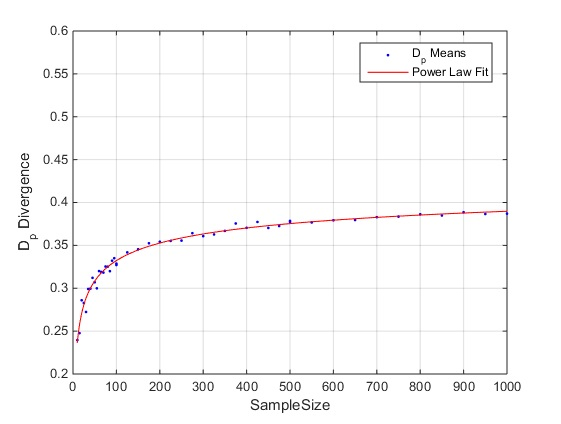
\includegraphics[scale=0.6]{dp_n200_uniform}
		%	\end{center}
	\end{figure}	
	
	\begin{figure}[h!]
		\caption{Distribution of $D_p$ Values for 8-Dimensional Uniform Data Set, N = 200 trials}
		\centering
		%	\begin{center}
		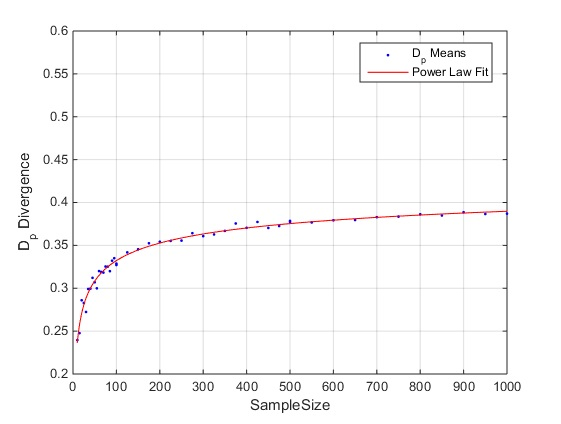
\includegraphics[scale=0.6]{dp_n200_uniform}
		%	\end{center}
	\end{figure}	

	\subsection*{\small Gaussian Dataset}
	
	\begin{table}[!h]
		\caption{Gaussian Dataset for Bootstrap Analysis of $D_p$}
		\centering % used for centering table
		\begin{tabular}{c c c c c c c c c c} % centered columns (4 columns)
			%inserts double horizontal lines
			$D_0$ &  &  &  \\ [0.5ex] % inserts table
			%heading
			\hline % inserts single horizontal line
			$\mu_0$ & 0 & 0 & 0 & 0 & 0 & 0 & 0 & 0\\[0.5ex] % inserting body of the table
			$\sigma_0$ & 1 & 1 & 1 & 1 & 1 & 1 & 1 & 1\\[0.5ex]
			
			$D_1$ & \\ [0.5ex]
			
			\hline
			$\mu_1$ & 0 & 0 & 0 & 0 & 0 & 0 & 0 & 0\\[0.5ex] % inserting body of the table
			$\sigma_1$ & 2.56 & 1 & 1 & 1 & 1 & 1 & 1 & 1\\[0.5ex]
			\hline %inserts single line
		\end{tabular}
		\label{table:nonlin} % is used to refer this table in the text
	\end{table}
	
	\begin{figure}[h!]
		\caption{Asymptotic Convergence of $D_p$ for Gaussian Data Set, N = 50 trials}
		\centering
		%	\begin{center}
		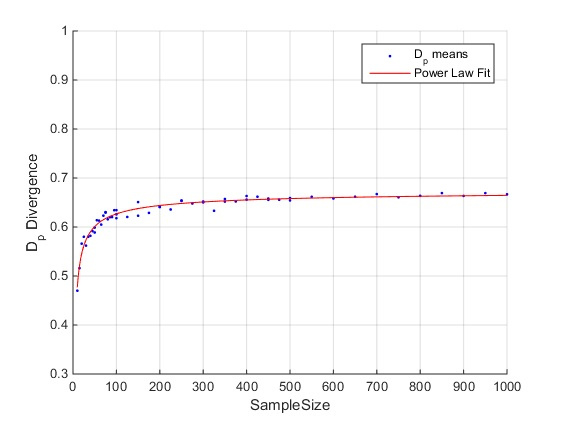
\includegraphics[scale=0.6]{dp_n50_gaussian}
		%	\end{center}
	\end{figure}	
	
	\newpage
	\subsection*{\small Banknote Dataset}
	The first real world example we consider is the Banknote Authentication Data Set taken from the University of California, Irvine Machine Learning Repository [7]. The 4-dimensional dataset contains data extracted from images of banknotes. The data set consists of a relatively small number of dimensions, and highly separated data, so the convergence is . We note that for a sensitive task such as authenticating banknotes, it should not be surprising to see an asymptotic value for $D_p$ that is close to 1.  
	
	\newpage
	\begin{figure}[h!]
		\caption{Convergence of $D_p$ for Banknote Authentication Data Set, N = 50 trials}
		\centering
		%	\begin{center}
		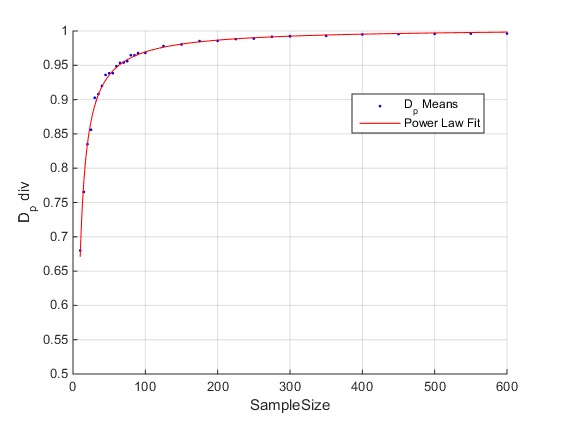
\includegraphics[scale=0.6]{dp_n50_banknote}
		%	\end{center}
	\end{figure}
	
	\newpage
	\subsection*{\small Pima Indians Dataset}
	
	\begin{figure}[!h]
		\caption{Asymptotic Convergence for Pima Indian Data Set, N = 50 trials}
		\centering
		%	\begin{center}
		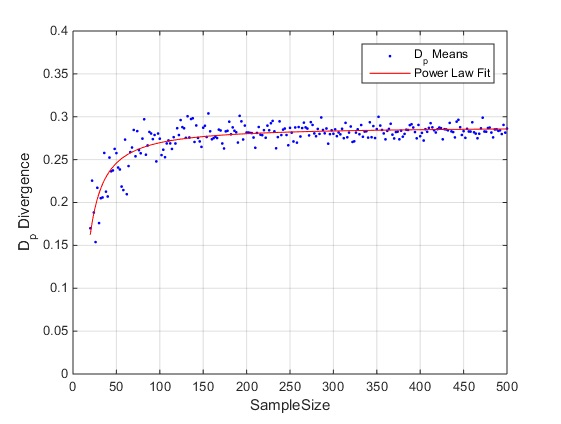
\includegraphics[scale=0.6]{dp_n50_pima}
		%	\end{center}
	\end{figure}
	
	\begin{figure}[!h]
		\caption{Asymptotic Convergence for Pima Indian Data Set, N = 200 trials}
		\centering
		%	\begin{center}
		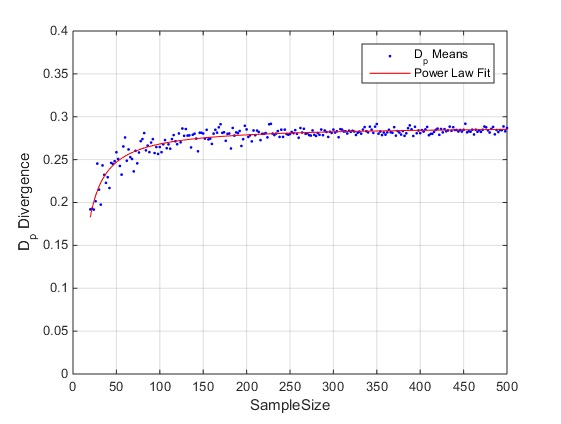
\includegraphics[scale=0.6]{dp_n200_pima}
		%	\end{center}
	\end{figure}	
	
	\begin{figure}[!h]
		\caption{Asymptotic Convergence for Pima Indian Data Set, N = 5000 trials}
		\centering
		%	\begin{center}
		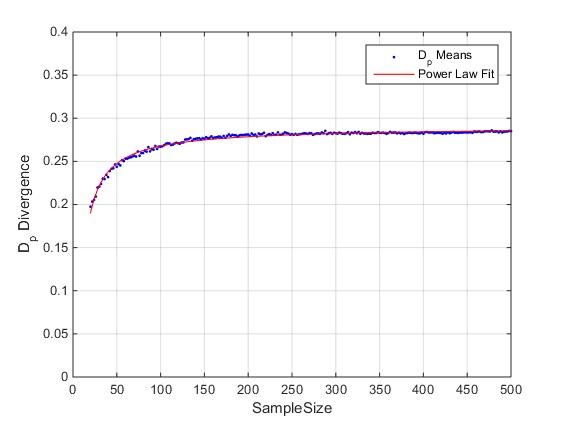
\includegraphics[scale=0.6]{dp_n5000}
		%	\end{center}
	\end{figure}	
	
	%		\begin{figure}[!h]
	%			\caption{Asymptotic Convergence for Pima Indian Data Set, N = 5000 trials}
	%			\centering
	%			%	\begin{center}
	%			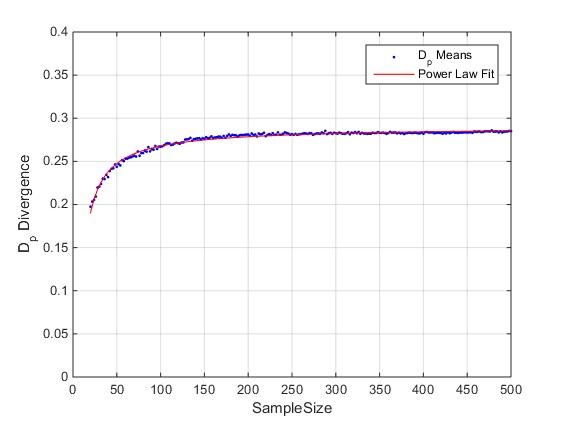
\includegraphics[scale=0.75]{dp_n5000}
	%			%	\end{center}
	%		\end{figure}	
	
	\newpage
	\begin{table}[!h]		
		\caption{Bayes Error Rates in Literature for Pima Indians Data Set [4]}
		\begin{center}
			%	\begin{tabular}{||c c c c||} 
			%		\hline
			\begin{tabular}[!h]{ |p{5cm}||p{4cm}|  }
				
				\hline
				Algorithm & Bayes Error Rate (\%) \\ [0.5ex] 
				\hline\hline
				
				Discrim & 22.50	\\
				Quadisc &  26.20	\\
				Logdisc &  22.30	\\
				SMART  & 23.20	\\
				ALLOC80 &  30.10	\\
				K-NN  & 32.40	\\
				CASTLE &  25.80	\\
				CART  & 25.50	\\
				IndCART &  27.10	\\
				NewID &  28.90	\\
				AC2 &  27.60	\\
				Baytree  & 27.10	\\
				NaiveBay &  26.20	\\
				CN2  & 28.90	\\
				C4.5  & 27.00	\\
				Itrule &  24.50	\\
				Cal5  & 25.00	\\
				Kohonen &  27.30	\\
				DIPOL92 &  22.40	\\
				Backprob  & 24.80	\\
				RBF  & 24.30	\\
				LVQ  & 27.20 	\\ 
				
		%		\textbf{$D_p$}  \\
		%		\textbf{$D_p$ Asymptotic Power Law} & \textbf{22.83} \\ 
				\hline 		
			\end{tabular}
		\end{center}
	\end{table}
	
	
		
	\begin{table}[!h]		
		\caption{Bootstrap Estimated Bayes Error Rates for Pima Indians Data Set [4]}
		\begin{center}
			%	\begin{tabular}{||c c c c||} 
			%		\hline
			\begin{tabular}[!h]{ |p{5cm}||p{4cm}|  }
				\hline
				Algorithm & Bayes Error Rate (\%) \\ [0.5ex] 
				\hline\hline
						$D_p$ (no Bootstrap) & $29.32 \pm 6.22$ * \\
						Efron Bootstrap  & $14.87 \pm 2.465$ ** 	\\
						$m < n$ Bootstrap, $m=200$ & $23.13 \pm 4.13$ 	\\
				\textbf{$D_p$ Asymptotic Power Law} & $\textbf{23.95} \pm \textbf{0.11}$\\ 
				\hline 		
			\end{tabular}
		\end{center}
	\end{table}
	
	\newpage
	\begin{table}[!h]		
		\caption{$D_p$ and Bayes Error Rate for the Pima Indian Data Set for Increasing Sample Size, and Increasing Monte Carlo Iterations}
		\begin{center}
			%	\begin{tabular}{||c c c c||} 
			%		\hline
			\begin{tabular}[!h]{ |p{2cm}||p{2cm}|p{5cm}|p{4cm}|  }
				
				\hline
				Sample Size & Monte Carlo Iterations & $D_p$ Asymptotic Value (95\% Confidence Interval)& Bayes Error Rate (\%), (95\% CI) \\ [0.5ex] 
				\hline\hline
				100	& 50	& 0.2725   (0.245, 0.3)	& $23.90  \pm 1.32$\\
				
				\hline
				
				100	& 200	& 0.2958  (0.265, 0.3267)	& $22.81  \pm 1.42$\\
				\hline
				
				100	& 5000	& 0.3107  (0.2959, 0.3254)	& $22.13  \pm 0.67$\\
				
				\hline
				200	& 50	& 0.2946  (0.2732, 0.3161)	& $22.86  \pm 0.99$\\
				
				\hline
				200	& 200	& 0.3029  (0.288, 0.3178)	& $22.48  \pm 0.68$\\
				
				\hline
				200	& 5000  & 0.3162  (0.3114, 0.3209)	& $21.88  \pm 0.21$\\
				
				\hline
				300	& 50	& 0.3118  (0.2827, 0.3409)  & $22.08  \pm 1.31$\\
				
				\hline
				300	& 200	& 0.3073  (0.2926, 0.3219)	& $22.28  \pm 0.66$\\
				\hline
				300	& 5000	& 0.3041  (0.3006, 0.3075)	& $22.43  \pm 0.16$\\ 
				\hline 		
			\end{tabular}
		\end{center}
	\end{table}			
	%	\newpage
	%		\section{Conclusion}
	
	\newpage
	\section*{References}[!h]
	[1] Hawes, Chad M., and Carey E. Priebe. "A Bootstrap Interval Estimator for Bayes' Classification Error." 2012 IEEE Statistical Signal Processing Workshop, 2012
	\\ [0.5ex]
	\noindent[2] V. Berisha, A. Wisler, A.O. Hero, and A. Spanias, "Empirically Estimable Classification Bounds Based on a Nonparametric Divergence Measure" IEEE Transactions on Signal Processing, vol. 64, no. 3, pp.580-591, Feb. 2016.
	\\ [0.5ex]
	\noindent[3] A. O. Hero, B. Ma, O. Michel, and J. Gorman, “Alpha-divergence for classification, indexing and retrieval,” Communication and Signal Processing Laboratory, Technical Report CSPL-328, U. Mich, 2001
	\\ [0.5ex]
	\noindent [4] K. Tumer, K. (1996) "Estimating the Bayes error rate through classifier combining" in Proceedings of the 13th International Conference on Pattern Recognition, Volume 2, 695–699
	
	Contains the pima indian dataset BERs in table format
	\\ [0.5ex]
	\noindent[5] Tumer, Kagan, and Joydeep Ghosh. "Bayes Error Rate Estimation Using Classifier Ensembles." International Journal of Smart Engineering System Design 5.2 (2003): 95-109.
	\\ [0.5ex]
	
	\noindent[6] Lichman, M. (2013). UCI Machine Learning Repository [http://archive.ics.uci.edu/ml]. Irvine, CA: University of California, School of Information and Computer Science.
	\\ [0.5ex]
	
	\noindent [7] V. Lohweg, “Banknote Authentication Data Set,” 2012. [Online]. Available: https://archive.ics.uci.edu/ml/datasets/banknote+authentication.
	\\ [0.5ex]
	
	\noindent [8] K. Pranesh, and L. Hunter. "On an Information Divergence Measure and Information Inequalities." (n.d.): n. pag. University of Northern British Columbia. 
	\\ [0.5ex]
	
	\noindent [9] Tukey, J.W. 1958. Bias and confidence in not-quite large samples. Annals of Mathematical Statistics 29: 614
	
	\noindent [10]Efron, B. "Bootstrap Methods: Another Look at the Jackknife." Annals of Statistics 7.1 (1979)
	
	
	\noindent [11] https://www.princeton.edu/~verdu/reprints/WanKulVerSep2005.pdf **Create Citation
	
	\noindent [12]http://www.princeton.edu/~verdu/reprints/WanKulVer.May2009.pdf?q=tilde/verdu/reprints/WanKulVer.May2009.pdf **Create Citation
	
	\noindent [13]http://www.eecs.berkeley.edu/~wainwrig/Papers/NguWaiJor10.pdf **Create Citation
	
	\noindent [14] http://www.stat.yale.edu/~arb4/publications_files/DistributionEstimationConsistentInTotalVariationAndInTwoTypesOfInformationDivergenceIEEEIT.pdf
	**Create Citation
	
	\noindent [15] http://www.tsc.uc3m.es/~fernando/bare_conf3.pdf **Create Citation
	
	\noindent [16] http://arxiv.org/pdf/1404.6230.pdf** Create Citation
\end{document}